\documentclass[11pt,a4paper]{article}
\usepackage[french]{babel}
\usepackage{fontspec}
\usepackage[margin=2.2cm]{geometry}
\usepackage{amsmath,amssymb,bm}
\usepackage{booktabs,graphicx,float,caption,subcaption}
\usepackage{xcolor,listings}
\usepackage[hidelinks]{hyperref}
\usepackage{enumitem}
\setlist{nosep,leftmargin=*}
\captionsetup{font=small,labelfont=bf}
\graphicspath{{../figures/}{figures/}}
\lstset{basicstyle=\ttfamily\footnotesize,frame=single,breaklines=true,keywordstyle=\color{blue!60!black},
  commentstyle=\color{gray},language=Python,columns=fullflexible}
\newcommand{\R}{\mathbb{R}}

\title{\textbf{Adaptation efficace de modèles de langage par LoRA}\\[0.3em]
\large Étude expérimentale de la méthode PEFT--LoRA sur la classification de sentiments}
\author{RAHANETRA Fanasina Jason\\
\small Master 1 Intelligence Artificielle et Big Data --- Python avancé\\
\small Enseignant : RATIARISON Tsinto Aina}
\date{Octobre 2026}

\begin{document}
\maketitle

\begin{abstract}
\noindent Le fine-tuning complet des modèles pré-entraînés met à jour tous leurs paramètres. Cela coûte cher en mémoire, en temps et en stockage, et devient vite impossible sur du matériel grand public. Nous étudions \emph{Low-Rank Adaptation} (LoRA), une méthode de \emph{Parameter-Efficient Fine-Tuning} (PEFT) qui gèle le modèle et n'apprend qu'une mise à jour de rang faible des matrices de poids. Nous implémentons LoRA à la main en PyTorch, nous la validons contre la bibliothèque Hugging~Face PEFT et nous la comparons au fine-tuning complet et à l'entraînement de la seule tête de classification. Les expériences portent sur DistilBERT et le jeu SST-2, sur une carte GeForce GTX~1050 de 4~Go. LoRA ($r=4$) atteint 89,1\,\% d'accuracy contre 89,3\,\% pour le fine-tuning complet, en n'entraînant que 0,98\,\% des paramètres, avec $44\,\%$ de mémoire GPU et $32\,\%$ de temps d'entraînement en moins et un checkpoint 90 fois plus léger (2,6~Mo contre 255~Mo). Une application web Gradio démontre l'utilisation du modèle adapté.
\end{abstract}

%=====================================================================
\section{Introduction}
%=====================================================================
\paragraph{Problème.} Les modèles de type Transformer \cite{vaswani2017} pré-entraînés sur de grands corpus s'adaptent ensuite à une tâche cible par \emph{fine-tuning}. La version classique, le fine-tuning complet, met à jour l'ensemble des $|\Theta|$ paramètres. Elle impose donc de garder en mémoire les poids, les gradients et les deux moments de l'optimiseur Adam, soit environ $4|\Theta|$ valeurs. Elle produit aussi une copie complète du modèle pour chaque tâche. Pour un modèle de 7~milliards de paramètres, cela représente plus de 100~Go de mémoire GPU pendant l'entraînement et 14~Go de stockage par tâche. Même un modèle « petit » comme DistilBERT (67~M de paramètres) remplit vite une carte de 4~Go. La question est donc la suivante : \emph{peut-on adapter un grand modèle à une nouvelle tâche en n'entraînant qu'une infime fraction de ses paramètres, sans perdre en performance~?}

\paragraph{État de l'art.} Les méthodes PEFT \cite{mangrulkar2022peft} se répartissent en trois familles :
\begin{itemize}
\item \textbf{Méthodes additives par modules} : les \emph{adapters} \cite{houlsby2019} insèrent de petits réseaux à goulot d'étranglement dans chaque bloc Transformer. Ils sont efficaces, mais ajoutent une latence à l'inférence, car les couches supplémentaires sont séquentielles.
\item \textbf{Méthodes par prompts appris} : \emph{prefix-tuning} \cite{li2021prefix} et \emph{prompt tuning} \cite{lester2021} apprennent des vecteurs ajoutés à l'entrée ou aux clés et valeurs de l'attention. Ils réduisent la longueur de séquence utile et sont difficiles à optimiser.
\item \textbf{Méthodes sélectives et reparamétrisations} : BitFit \cite{benzaken2021} n'entraîne que les biais. \textbf{LoRA} \cite{hu2021lora} repose sur l'observation qu'un modèle pré-entraîné a une faible \emph{dimension intrinsèque} \cite{aghajanyan2020} : la mise à jour utile des poids peut être de rang faible. LoRA apprend donc $\Delta W = BA$ de rang $r$ et peut la \emph{fusionner} dans $W_0$ après l'entraînement, sans aucun surcoût à l'inférence.
\end{itemize}
LoRA a depuis donné de nombreuses variantes : QLoRA \cite{dettmers2023qlora} (modèle de base quantifié en 4~bits), AdaLoRA \cite{zhang2023adalora} (rang alloué dynamiquement) et DoRA \cite{liu2024dora} (décomposition en amplitude et direction). C'est aujourd'hui la méthode d'adaptation la plus utilisée pour les grands modèles de langage.

\paragraph{Contributions.} (i) Une implémentation pédagogique de LoRA en PyTorch, vérifiée par des tests unitaires (équivalence à l'initialisation et après fusion). (ii) Une comparaison chiffrée et \emph{profilée} (temps, mémoire GPU, débit, taille sur disque) entre le fine-tuning complet, la tête seule et LoRA pour plusieurs rangs. (iii) Une application web fonctionnelle (Gradio) qui sert le modèle adapté.

%=====================================================================
\section{Méthodologie}
%=====================================================================
\subsection{Description technique}
\paragraph{Modèle et tâche.} Nous utilisons \texttt{distilbert-base-uncased} \cite{sanh2019distilbert}. Ce modèle comporte $L=6$ blocs Transformer de dimension $d=768$, 12 têtes d'attention et une couche intermédiaire de 3072 neurones. La tâche est la classification binaire de sentiments sur SST-2 \cite{socher2013sst,wang2018glue} : des phrases de critiques de films étiquetées positives ou négatives. Nous utilisons 20\,000 phrases d'entraînement tirées aléatoirement (graine 42) et les 872 phrases du jeu de validation officiel. La tête de classification est composée d'une couche dense $768\to768$ (\texttt{pre\_classifier}) puis d'une couche $768\to2$.

\paragraph{Méthodes comparées.}
\begin{enumerate}
\item \textbf{Fine-tuning complet} : tous les paramètres sont entraînés.
\item \textbf{Tête seule} (\emph{linear probing}) : l'encodeur est gelé et seule la tête est entraînée. C'est la borne basse en nombre de paramètres.
\item \textbf{LoRA (PEFT)} : des adaptateurs sont placés sur les projections $W_q$ et $W_v$ de l'attention dans les 6 blocs, comme dans \cite{hu2021lora}, avec $r\in\{4,8,16\}$, $\alpha=16$ et un dropout de $0{,}1$. La tête reste entraînable.
\item \textbf{LoRA maison} ($r=8$) : notre implémentation (classe \texttt{LoRALinear}), avec la même configuration que PEFT.
\end{enumerate}

\paragraph{Implémentation.} Le code est en Python~3.12 avec PyTorch~2.5.1 (CUDA~12.1), Transformers~4.46, PEFT~0.13 et Datasets~3.1. La boucle d'entraînement est écrite à la main pour contrôler le profilage. Un gestionnaire de contexte \texttt{Timer.section} synchronise le GPU avant de mesurer le temps, et les pics mémoire sont relevés avec \texttt{torch.cuda.max\_memory\_allocated}. L'optimiseur est AdamW (décroissance des poids $0{,}01$), avec un \emph{warmup} linéaire sur 6\,\% des pas puis une décroissance linéaire. Nous faisons 2 époques avec des lots de 32 et des séquences tronquées à 128 jetons, complétées dynamiquement. Les taux d'apprentissage sont $2\cdot10^{-5}$ pour le fine-tuning complet, $5\cdot10^{-4}$ pour LoRA et $10^{-3}$ pour la tête seule. Le cœur de l'implémentation est le suivant :
\begin{lstlisting}
class LoRALinear(nn.Module):
    def __init__(self, base: nn.Linear, r=8, alpha=16.0, dropout=0.0):
        super().__init__()
        self.base = base; self.base.weight.requires_grad_(False)   # W0 gele
        self.scaling = alpha / r
        self.lora_A = nn.Parameter(torch.empty(r, base.in_features))
        self.lora_B = nn.Parameter(torch.zeros(base.out_features, r))  # B = 0
        nn.init.kaiming_uniform_(self.lora_A, a=math.sqrt(5))
    def forward(self, x):
        return self.base(x) + (self.dropout(x) @ self.lora_A.T @ self.lora_B.T) * self.scaling
\end{lstlisting}

\subsection{Formulation mathématique}
\paragraph{Fine-tuning complet.} Soit un jeu $\mathcal{D}=\{(x_i,y_i)\}_{i=1}^N$, avec $y_i\in\{0,1\}$, et un modèle $f_\Theta$ qui produit des logits $\bm{z}=f_\Theta(x)\in\R^{C}$, où $C=2$. Le fine-tuning complet résout
\begin{equation}
\Theta^\star=\arg\min_{\Theta}\ \mathcal{L}(\Theta),\qquad
\mathcal{L}(\Theta)=-\frac{1}{N}\sum_{i=1}^{N}\log\frac{\exp\big(z_{i,y_i}\big)}{\sum_{c=1}^{C}\exp\big(z_{i,c}\big)} ,
\label{eq:ce}
\end{equation}
à partir de $\Theta_0$ pré-entraîné. Tous les paramètres reçoivent un gradient.

\paragraph{Reparamétrisation LoRA.} Pour une couche linéaire $h=W_0x$, avec $W_0\in\R^{d\times k}$, LoRA gèle $W_0$ et contraint la mise à jour à être de rang au plus $r\ll\min(d,k)$ :
\begin{equation}
h \;=\; W_0x+\Delta W x \;=\; W_0x+\frac{\alpha}{r}\,B A\,x,\qquad B\in\R^{d\times r},\; A\in\R^{r\times k}.
\label{eq:lora}
\end{equation}
Le facteur $\alpha/r$ découple l'amplitude de la mise à jour du choix de $r$ : on peut changer $r$ sans réajuster le taux d'apprentissage. On initialise $A_{ij}\sim\mathcal{U}\!\left(-\tfrac{1}{\sqrt{k}},\tfrac{1}{\sqrt{k}}\right)$ et $B=\bm{0}$, si bien que
\begin{equation}
\Delta W\big|_{t=0}=BA=\bm{0}\quad\Longrightarrow\quad f_{\Theta_0+\Delta\Theta}(x)=f_{\Theta_0}(x)\ \text{au départ.}
\end{equation}
Le calcul se fait comme $\big((xA^\top)B^\top\big)$ : la matrice $d\times k$ n'est jamais matérialisée, et le coût supplémentaire n'est que de $\mathcal{O}\big(r(d+k)\big)$ par jeton.

\paragraph{Gradients.} En notant $G=\partial\mathcal{L}/\partial h$ et $s=\alpha/r$, la règle de dérivation en chaîne donne
\begin{equation}
\frac{\partial\mathcal{L}}{\partial W_0}\ \text{non calculé (gelé)},\qquad
\frac{\partial\mathcal{L}}{\partial B}=s\,G\,(Ax)^\top,\qquad
\frac{\partial\mathcal{L}}{\partial A}=s\,B^\top G\,x^\top .
\end{equation}
Au premier pas, $B=\bm 0$, donc $\partial\mathcal L/\partial A=\bm 0$ : seul $B$ évolue d'abord, ce qui rend le début de l'entraînement stable.

\paragraph{Nombre de paramètres.} Pour une matrice, LoRA entraîne $r(d+k)$ paramètres au lieu de $dk$, soit un ratio de
\begin{equation}
\rho=\frac{r(d+k)}{dk}\;\overset{d=k=768,\;r=8}{=}\;\frac{8\cdot1536}{768^2}\approx2{,}08\,\%.
\end{equation}
Sur DistilBERT, avec $W_q$ et $W_v$ adaptées dans les $L=6$ blocs, on a
\begin{equation}
|\Theta_{\text{LoRA}}|=2L\,r\,(d+k)=12\cdot r\cdot1536=18\,432\,r,
\qquad |\Theta_{\text{tête}}|=(768^2+768)+(768\cdot2+2)=592\,130 .
\end{equation}
Pour $r=8$, cela donne $147\,456+592\,130=739\,586$ paramètres entraînables sur $67{,}1$~M, soit $1{,}10\,\%$. Ce chiffre est confirmé par l'exécution (section~\ref{sec:res}).

\paragraph{Mémoire.} En précision simple (4 octets) avec AdamW, qui garde deux moments $m_t$ et $v_t$, la mémoire statique est d'environ
\begin{equation}
M_{\text{statique}}\approx 4\,\big(|\Theta| + \underbrace{|\Theta_{\text{tr}}|}_{\text{gradients}} + \underbrace{2|\Theta_{\text{tr}}|}_{m_t,\,v_t}\big)\ \text{octets},
\end{equation}
auquel s'ajoutent les activations. Le fine-tuning complet ($|\Theta_{\text{tr}}|=|\Theta|$) coûte $16|\Theta|\approx1{,}07$~Go, contre $\approx0{,}28$~Go pour LoRA.

\paragraph{Mise à jour AdamW.} Pour chaque paramètre entraînable $\theta$, avec le gradient $g_t$ :
\begin{equation}
m_t=\beta_1m_{t-1}+(1-\beta_1)g_t,\quad v_t=\beta_2v_{t-1}+(1-\beta_2)g_t^2,\quad
\theta_t=\theta_{t-1}-\eta_t\Big(\frac{\hat m_t}{\sqrt{\hat v_t}+\epsilon}+\lambda\theta_{t-1}\Big),
\end{equation}
avec $\hat m_t=m_t/(1-\beta_1^t)$, $\hat v_t=v_t/(1-\beta_2^t)$ et le taux d'apprentissage
\begin{equation}
\eta_t=\eta_{\max}\cdot\begin{cases} t/T_w & t<T_w\\[2pt] \dfrac{T-t}{T-T_w} & t\ge T_w\end{cases},\qquad T_w=\lfloor0{,}06\,T\rfloor .
\end{equation}

\paragraph{Fusion pour l'inférence.} Après l'entraînement, on calcule une seule fois
\begin{equation}
W=W_0+\frac{\alpha}{r}BA ,
\end{equation}
et l'on obtient un modèle de même architecture que l'original, sans \emph{aucune latence ajoutée}. Pour changer de tâche, il suffit de soustraire $\frac{\alpha}{r}BA$ et d'ajouter un autre adaptateur.

\paragraph{Métriques.} Avec $TP$, $TN$, $FP$ et $FN$ les vrais et faux positifs et négatifs :
\begin{equation}
\text{Acc}=\frac{TP+TN}{TP+TN+FP+FN},\quad P=\frac{TP}{TP+FP},\quad R=\frac{TP}{TP+FN},\quad F_1=\frac{2PR}{P+R}.
\end{equation}
Pour le profilage, nous mesurons la durée d'entraînement $T_{\text{train}}$, le débit $\frac{E\cdot N}{T_{\text{train}}}$ (en échantillons par seconde, avec $E$ le nombre d'époques), le pic de mémoire GPU et la taille du checkpoint sauvegardé.

%=====================================================================
\section{Résultats et discussion}\label{sec:res}
%=====================================================================
\subsection{Contexte expérimental}
Les six configurations ont été entraînées l'une après l'autre sur la même machine, avec les mêmes 20\,000 phrases, le même ordre de lots (graine 42) et les mêmes hyperparamètres (2 époques, soit $T=1250$ pas). Les métriques sont mesurées sur les 872 phrases de validation de SST-2, dont 428 négatives et 444 positives. Toutes les durées sont mesurées après synchronisation CUDA (\texttt{torch.cuda.synchronize}). La mémoire est le pic alloué par PyTorch sur le GPU pendant l'entraînement. L'ensemble des expériences est reproductible avec la commande \texttt{./run\_experiments.sh}.

\subsection{Configuration de l'ordinateur}
\begin{table}[H]\centering\small
\begin{tabular}{ll}\toprule
Processeur & Intel Core i5-8300H @ 2,30~GHz (4 cœurs physiques / 8 logiques)\\
Mémoire vive & 15,3~Go\\
GPU & NVIDIA GeForce GTX~1050, 4~Go GDDR5 (architecture Pascal, capacité de calcul 6.1)\\
Pilote / CUDA & NVIDIA 535.309 / CUDA~12.1 (runtime PyTorch)\\
Système & Linux (noyau 7.0), Python~3.12.9\\
Bibliothèques & PyTorch~2.5.1, Transformers~4.46.3, PEFT~0.13.2, Datasets~3.1.0, Gradio~5.9.1\\
\bottomrule\end{tabular}
\caption{Matériel et logiciels utilisés. La GTX~1050 n'est plus prise en charge par PyTorch $\geq2.6$. Sur cette architecture, le calcul en fp16 est très lent, d'où l'entraînement en fp32.}
\end{table}

\subsection{Performances de classification}
\begin{table}[H]\centering
\resizebox{\textwidth}{!}{\begin{tabular}{lrrrrrrrr}
\toprule
Méthode & Param. entr. & \% & Acc. & F1 & Durée (min) & Éch./s & GPU (Mo) & Disque (Mo) \\
\midrule
Tête seule & 592\,130 & 0{,}88 & 83{,}14 & 83{,}58 & 2{,}9 & 229 & 393 & 255{,}43 \\
LoRA r=4 & 665\,858 & 0{,}98 & 89{,}11 & 89{,}31 & 5{,}0 & 132 & 800 & 2{,}55 \\
LoRA r=8 & 739\,586 & 1{,}09 & 88{,}19 & 88{,}72 & 5{,}0 & 132 & 804 & 2{,}83 \\
LoRA r=16 & 887\,042 & 1{,}31 & 88{,}88 & 89{,}26 & 5{,}0 & 132 & 806 & 3{,}39 \\
LoRA maison r=8 & 739\,586 & 1{,}10 & 88{,}07 & 88{,}34 & 5{,}0 & 132 & 801 & 2{,}83 \\
Fine-tuning complet & 66\,955\,010 & 100{,}00 & 89{,}33 & 89{,}77 & 7{,}4 & 90 & 1442 & 255{,}43 \\
\bottomrule
\end{tabular}}
\caption{Synthèse des six expériences. « \% » : part des paramètres entraînés. Acc. et F1 en \% sur la validation SST-2. Éch./s : débit d'entraînement. GPU : pic mémoire à l'entraînement. Disque : taille du checkpoint sauvegardé.}
\label{tab:res}
\end{table}

\begin{figure}[H]\centering
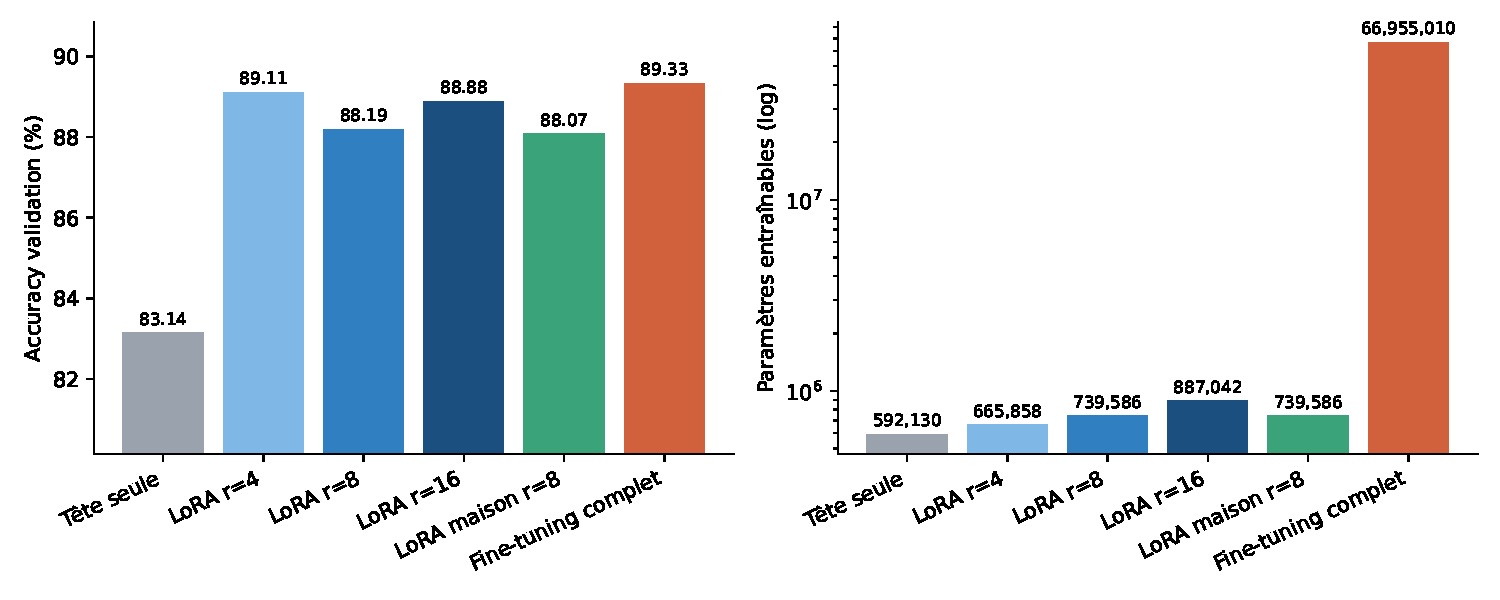
\includegraphics[width=\textwidth]{accuracy_params.pdf}
\caption{Gauche : accuracy de validation. Droite : nombre de paramètres entraînables (échelle logarithmique).}
\label{fig:acc}
\end{figure}

Le tableau~\ref{tab:res} et la figure~\ref{fig:acc} conduisent à trois constats.
\begin{enumerate}
\item \textbf{LoRA approche le fine-tuning complet avec environ 90 fois moins de paramètres.} La meilleure configuration LoRA ($r=4$, 89,11\,\%) est à $0{,}22$ point du fine-tuning complet (89,33\,\%) tout en n'entraînant que $0{,}98\,\%$ des paramètres.
\item \textbf{Adapter l'encodeur est indispensable.} Entraîner seulement la tête plafonne à 83,14\,\%. Avec à peine $73\,728$ paramètres LoRA de plus ($r=4$), on gagne $+6$ points. C'est bien la petite mise à jour $\Delta W$ des matrices d'attention qui apporte l'adaptation.
\item \textbf{Le rang a peu d'influence.} Les écarts entre $r=4$, $8$ et $16$ (88,2 à 89,1\,\%) sont inférieurs au bruit statistique. Pour une accuracy $p\approx0{,}89$ mesurée sur $n=872$ exemples, l'intervalle de confiance à 95\,\% vaut
\begin{equation}
\text{IC}_{95\,\%}=\hat p\pm1{,}96\sqrt{\frac{\hat p(1-\hat p)}{n}}\approx\hat p\pm2{,}1\ \text{points}.
\end{equation}
Toutes les variantes LoRA et le fine-tuning complet sont donc \emph{statistiquement équivalentes}, ce qui rejoint l'observation de \cite{hu2021lora} : un très petit rang suffit.
\end{enumerate}
Notre \textbf{LoRA maison} (88,07\,\%) et celle de \textbf{PEFT} (88,19\,\%), toutes deux de rang 8, ont exactement le même nombre de paramètres entraînables (739\,586, comme prévu par l'équation de la section~2) et des courbes d'apprentissage comparables. Cela valide notre implémentation. Le total légèrement plus élevé chez PEFT (67,69~M contre 67,10~M) vient de la copie de la tête qu'il conserve (\texttt{modules\_to\_save}). Les matrices de confusion sont équilibrées. Pour LoRA $r=4$ : $\left(\begin{smallmatrix}380&48\\47&397\end{smallmatrix}\right)$, soit autant de faux positifs que de faux négatifs.

\subsection{Profilage : durée, mémoire et stockage}
\begin{figure}[H]\centering
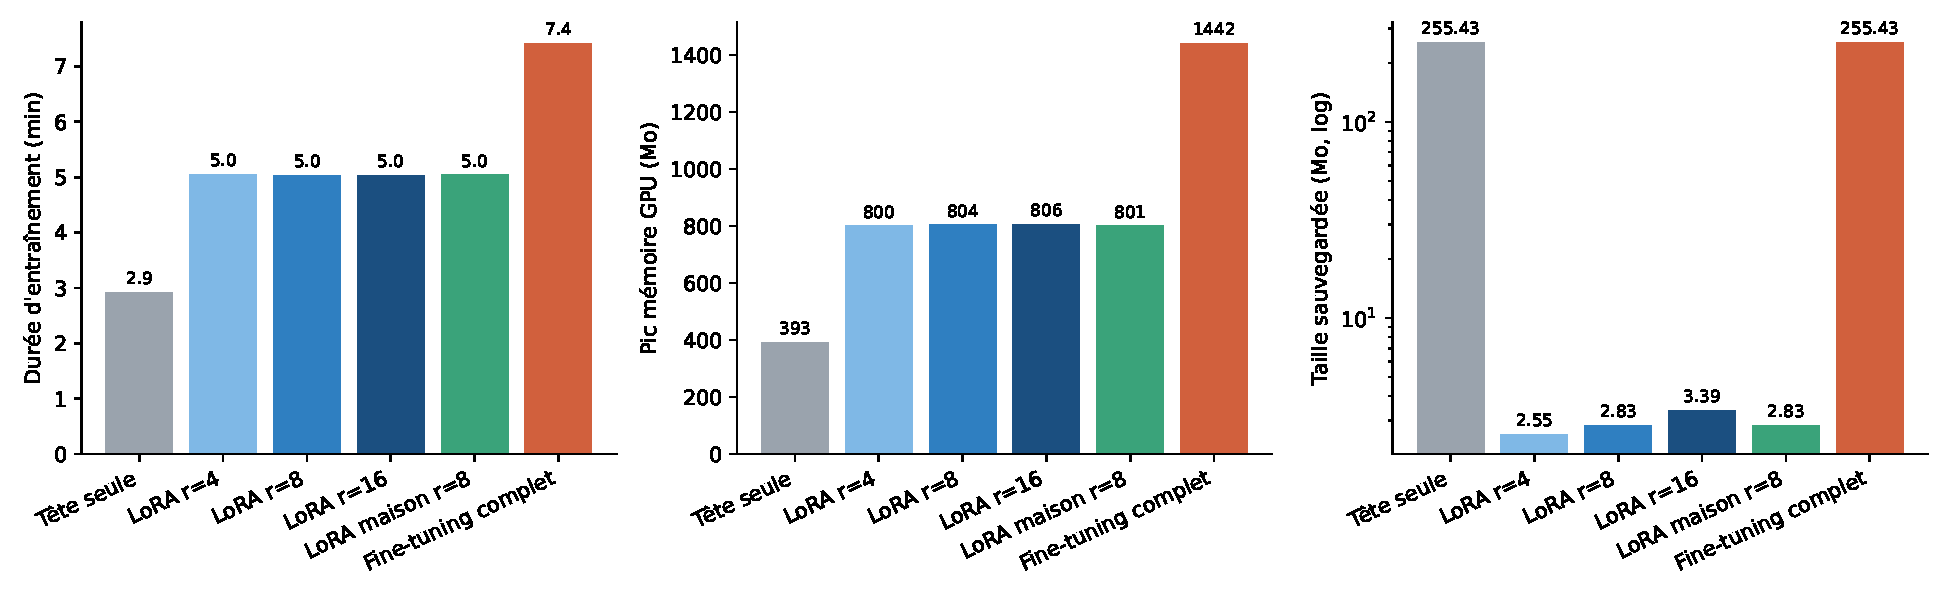
\includegraphics[width=\textwidth]{profiling.pdf}
\caption{Profilage mesuré sur la GTX~1050. Gauche : durée d'entraînement (2 époques). Centre : pic de mémoire GPU. Droite : taille sauvegardée (échelle logarithmique).}
\label{fig:prof}
\end{figure}

\paragraph{Durée d'entraînement.} Une époque prend 83~s pour la tête seule, 146~s pour LoRA (quel que soit $r$) et 218~s pour le fine-tuning complet. Le débit est respectivement de 229, 132 et 90 échantillons par seconde, soit environ 3\,040, 1\,760 et 1\,190 jetons par seconde. La préparation des données (tokenisation) prend environ 13~s. Le gain de LoRA ($-32\,\%$) s'explique par un modèle de coût simple. Si la passe avant coûte $F$, la rétropropagation coûte $\approx2F$ : $F$ pour les gradients des activations et $F$ pour ceux des poids. LoRA doit encore propager les gradients à travers l'encodeur gelé, mais ne calcule plus les gradients des poids $W_0$ :
\begin{equation}
\frac{T_{\text{LoRA}}}{T_{\text{full}}}\approx\frac{F+F}{F+2F}=\frac23\approx0{,}67
\qquad\text{contre}\qquad \frac{302{,}2\ \text{s}}{445{,}4\ \text{s}}=0{,}68\ \text{mesuré.}
\end{equation}
La tête seule n'a pas de rétropropagation dans l'encodeur ($\approx F$), d'où un rapport de $0{,}39$ mesuré, pour $1/3$ attendu. La différence vient de la tokenisation et des transferts, qui ne dépendent pas de la méthode.

\paragraph{Mémoire GPU.} Le pic passe de 1\,442~Mo (fine-tuning complet) à environ 804~Mo (LoRA), soit $-44\,\%$. Cela concorde avec l'équation de la mémoire statique : $16|\Theta|\approx1{,}07$~Go en fine-tuning complet, contre $\approx0{,}28$~Go pour LoRA. Les activations conservées pour la rétropropagation ajoutent environ 0,4 à 0,5~Go dans les deux cas. La tête seule (393~Mo) n'a presque pas d'activations à garder. Le rang a un effet négligeable (800 à 806~Mo), car les matrices $A$ et $B$ ne pèsent que quelques centaines de kilooctets.

\paragraph{Stockage.} Le fine-tuning complet produit un checkpoint de 255~Mo par tâche. Un adaptateur LoRA, tête comprise, pèse 2,8~Mo, soit \textbf{90 fois moins}. Un seul modèle de base peut ainsi servir des dizaines de tâches. Le checkpoint de la tête seule pèse lui aussi 255~Mo, car nous l'avons sauvegardé avec \texttt{save\_pretrained}, qui écrit tout le modèle. Seuls 2,3~Mo y sont réellement spécifiques à la tâche.

\paragraph{Inférence.} Après fusion $W=W_0+\frac{\alpha}{r}BA$, le modèle LoRA a exactement l'architecture de DistilBERT. L'évaluation des 872 phrases prend environ 4,9~s pour toutes les méthodes, et la latence d'une phrase dans l'application est d'environ 34~ms sur la GTX~1050. LoRA n'ajoute donc \emph{aucune} latence.

\begin{figure}[H]\centering
\begin{subfigure}{0.56\textwidth}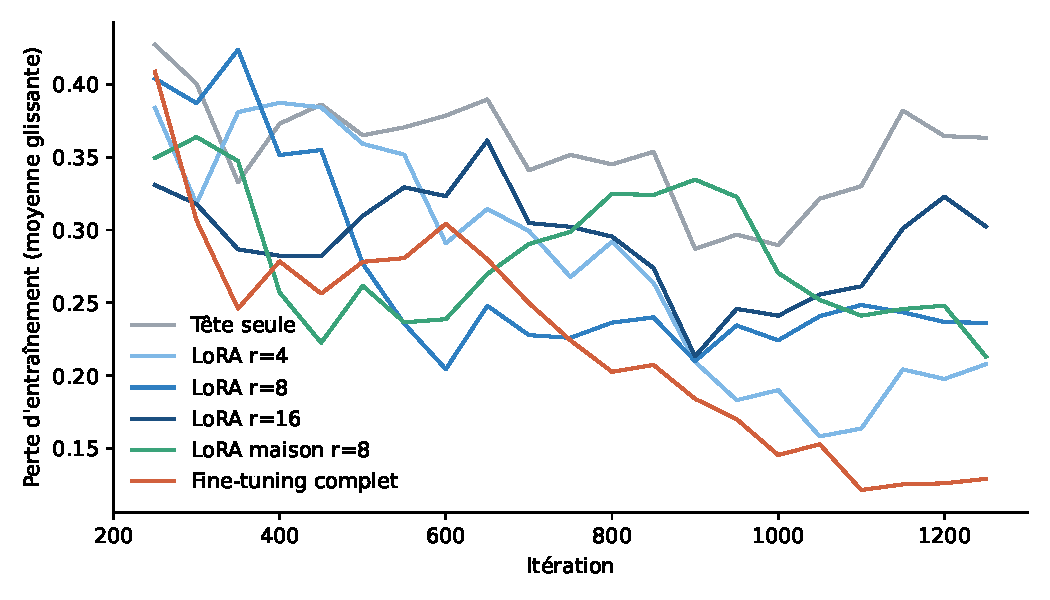
\includegraphics[width=\textwidth]{loss_curves.pdf}\caption{Perte d'entraînement (moyenne glissante sur 5 points).}\end{subfigure}\hfill
\begin{subfigure}{0.40\textwidth}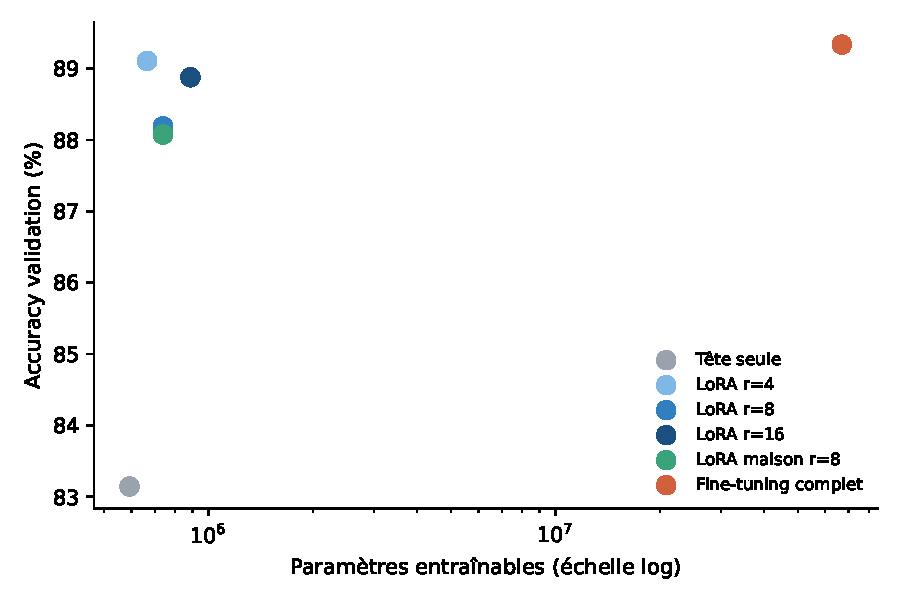
\includegraphics[width=\textwidth]{tradeoff.pdf}\caption{Compromis précision et paramètres.}\end{subfigure}
\caption{Dynamique d'apprentissage et compromis.}
\label{fig:loss}
\end{figure}

\paragraph{Dynamique d'apprentissage.} Le fine-tuning complet atteint la perte d'entraînement la plus basse ($\approx0{,}13$ en fin d'entraînement, contre $0{,}2$ à $0{,}3$ pour LoRA), sans meilleure accuracy de validation. La contrainte de rang faible agit donc comme une \emph{régularisation} : LoRA mémorise moins le jeu d'entraînement pour une généralisation équivalente. La tête seule reste au-dessus de $0{,}3$, faute de capacité.

\begin{figure}[H]\centering
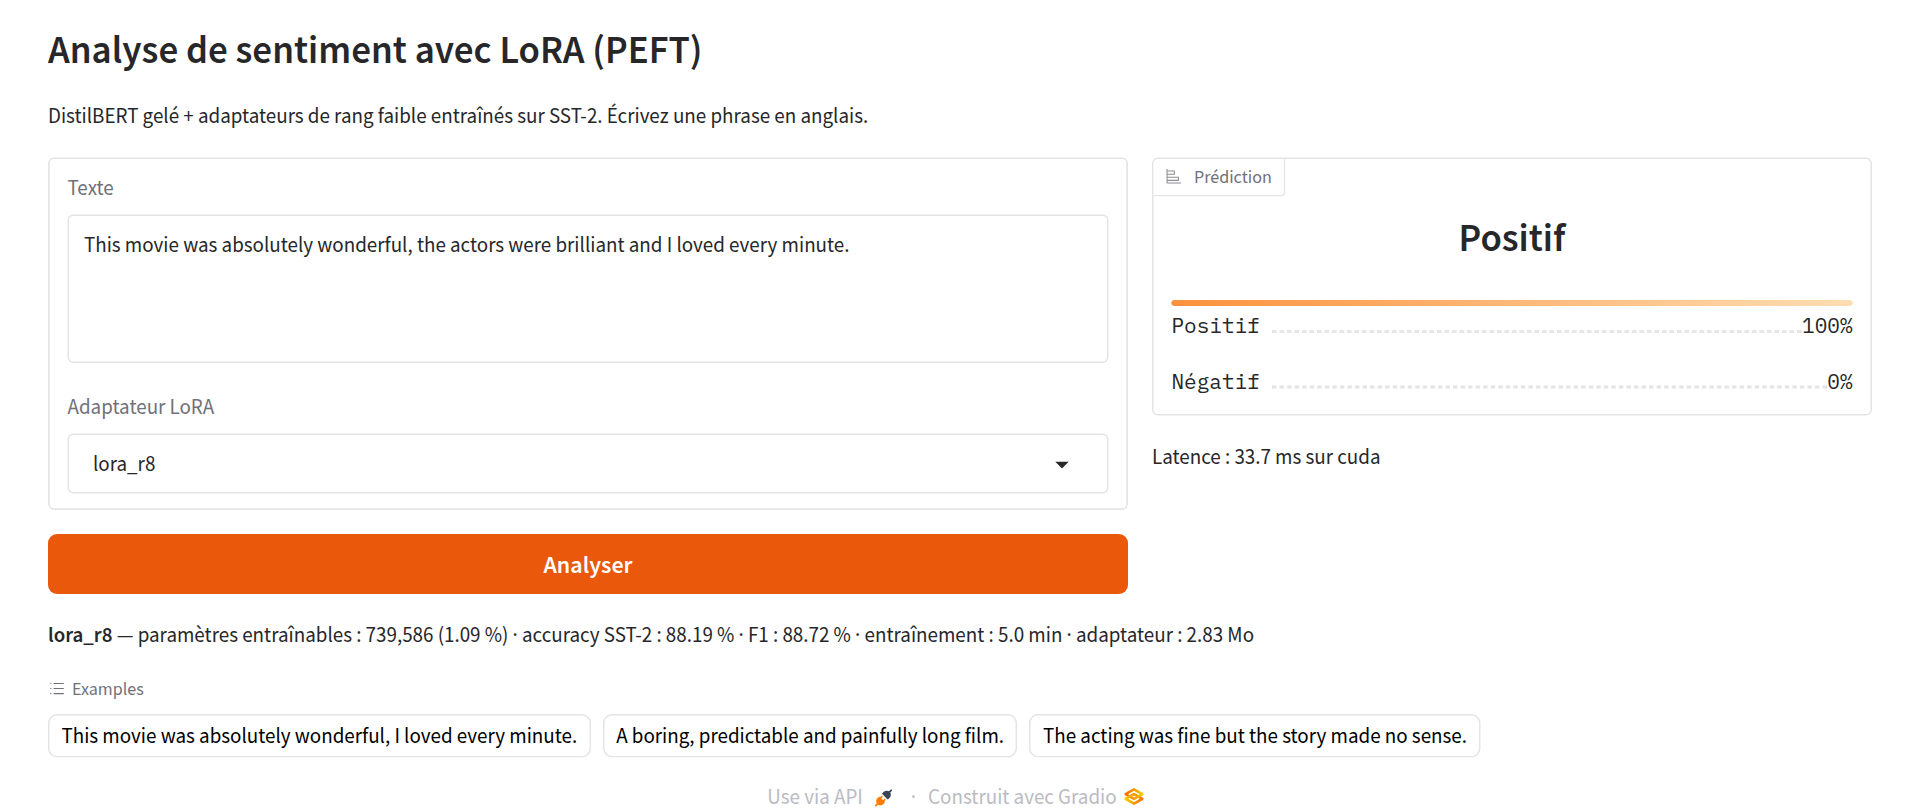
\includegraphics[width=0.92\textwidth]{app_screenshot.png}
\caption{Capture d'écran de l'application Gradio (\texttt{python app.py}) : l'adaptateur LoRA $r=8$ est fusionné dans DistilBERT et classe la phrase saisie, avec la latence et les métriques du modèle.}
\label{fig:app}
\end{figure}

\begin{figure}[H]\centering
\begin{lstlisting}[language={},basicstyle=\ttfamily\scriptsize]
$ python -m src.train --method lora --rank 8
INFO [lora_r8] paramètres entraînables : 739,586 / 67,694,596 (1.093 %)
INFO [lora_r8] epoch 1 step 200/1250 loss 0.2919
INFO [lora_r8] epoch 1 - val acc 0.8739 f1 0.8810
INFO [lora_r8] epoch 2 - val acc 0.8819 f1 0.8872
INFO [lora_r8] terminé en 302.2 s - acc 0.8819 - pic GPU 804 Mo
\end{lstlisting}
\caption{Extrait du journal d'entraînement de LoRA $r=8$ (fichier \texttt{results\_log.txt}).}
\end{figure}

\paragraph{Limites.} (i) Une seule graine par configuration : les écarts de moins de 2 points ne sont pas significatifs. (ii) La tâche est simple (classification binaire) et le modèle petit. Les gains relatifs de LoRA augmentent avec la taille du modèle, puisque la mémoire de l'optimiseur devient alors dominante. (iii) Les taux d'apprentissage n'ont pas été optimisés séparément pour chaque méthode.

%=====================================================================
\section{Conclusion}
%=====================================================================
Ce projet a implémenté, validé et profilé la méthode LoRA. En gelant DistilBERT et en n'apprenant que des mises à jour de rang $r\le16$ sur $W_q$ et $W_v$, nous obtenons une accuracy statistiquement équivalente au fine-tuning complet sur SST-2 (89,1\,\% contre 89,3\,\%). Le coût est nettement plus faible : 1\,\% des paramètres, $-44\,\%$ de mémoire GPU, $-32\,\%$ de temps d'entraînement et un checkpoint 90 fois plus léger. L'écart de temps mesuré correspond au modèle théorique $2/3$, et notre implémentation à la main reproduit les résultats de la bibliothèque PEFT. L'application Gradio montre qu'un adaptateur fusionné s'utilise exactement comme le modèle d'origine, sans latence supplémentaire.

\paragraph{Perspectives.} Appliquer QLoRA \cite{dettmers2023qlora} pour adapter un LLM génératif sur la même carte de 4~Go. Étendre LoRA à toutes les couches linéaires et comparer avec AdaLoRA et DoRA. Répéter les mesures sur plusieurs graines pour obtenir des intervalles de confiance.


\begin{thebibliography}{99}\small
\bibitem{vaswani2017} A. Vaswani et al., « Attention Is All You Need », \emph{NeurIPS}, 2017.
\bibitem{houlsby2019} N. Houlsby et al., « Parameter-Efficient Transfer Learning for NLP », \emph{ICML}, 2019.
\bibitem{li2021prefix} X. L. Li, P. Liang, « Prefix-Tuning: Optimizing Continuous Prompts for Generation », \emph{ACL}, 2021.
\bibitem{lester2021} B. Lester, R. Al-Rfou, N. Constant, « The Power of Scale for Parameter-Efficient Prompt Tuning », \emph{EMNLP}, 2021.
\bibitem{benzaken2021} E. Ben Zaken, S. Ravfogel, Y. Goldberg, « BitFit: Simple Parameter-efficient Fine-tuning for Transformer-based Masked Language-models », \emph{ACL}, 2022.
\bibitem{aghajanyan2020} A. Aghajanyan, L. Zettlemoyer, S. Gupta, « Intrinsic Dimensionality Explains the Effectiveness of Language Model Fine-Tuning », \emph{ACL}, 2021.
\bibitem{hu2021lora} E. J. Hu et al., « LoRA: Low-Rank Adaptation of Large Language Models », \emph{ICLR}, 2022.
\bibitem{dettmers2023qlora} T. Dettmers et al., « QLoRA: Efficient Finetuning of Quantized LLMs », \emph{NeurIPS}, 2023.
\bibitem{zhang2023adalora} Q. Zhang et al., « AdaLoRA: Adaptive Budget Allocation for Parameter-Efficient Fine-Tuning », \emph{ICLR}, 2023.
\bibitem{liu2024dora} S.-Y. Liu et al., « DoRA: Weight-Decomposed Low-Rank Adaptation », \emph{ICML}, 2024.
\bibitem{mangrulkar2022peft} S. Mangrulkar et al., « PEFT: State-of-the-art Parameter-Efficient Fine-Tuning methods », Hugging Face, 2022.
\bibitem{sanh2019distilbert} V. Sanh et al., « DistilBERT, a distilled version of BERT: smaller, faster, cheaper and lighter », 2019.
\bibitem{socher2013sst} R. Socher et al., « Recursive Deep Models for Semantic Compositionality Over a Sentiment Treebank », \emph{EMNLP}, 2013.
\bibitem{wang2018glue} A. Wang et al., « GLUE: A Multi-Task Benchmark and Analysis Platform for NLU », \emph{ICLR}, 2019.
\end{thebibliography}
\end{document}
